\documentclass[12pt, a4paper, oneside]{ctexbook}
\usepackage{amsmath, amsthm, amssymb, bm, graphicx, hyperref, mathrsfs, verbatim,tikz, makecell, longtable, xcolor, tcolorbox, soul, adjustbox, enumerate, pdfpages, float, colortbl, tabularx, multirow, pgfplots, underscore, listings, minted, circuitikz}
\numberwithin{figure}{section}
\title{{\Huge{\textbf{嵌入式开发}}}}
\author{Boyuan Zhao}
\date{\today}
\linespread{1.5}
\newtheorem{theorem}{定理}[section]
\newtheorem{definition}[theorem]{定义}
\newtheorem{lemma}[theorem]{引理}
\newtheorem{corollary}[theorem]{推论}
\newtheorem{example}[theorem]{例}
\newtheorem{proposition}[theorem]{命题}

\begin{document}

\maketitle

\pagenumbering{roman}
\setcounter{page}{1}

\begin{center}
    \Huge\textbf{前言}
\end{center}~\

临时抱佛脚. 
~\
\begin{flushright}
    \begin{tabular}{c}
        Boyuan Zhao\
        \today
    \end{tabular}
\end{flushright}

\newpage
\pagenumbering{Roman}
\setcounter{page}{1}
\tableofcontents

\newpage
\setcounter{page}{1}
\pagenumbering{arabic}

\chapter{嵌入式系统概述}
\section{嵌入式技术概念}
\textbf{狭义概念}:嵌入到对象体中的专用计算机系统

\textbf{三要素}:嵌入、专用、计算机

\textbf{嵌入式系统的特点}:由三要素引出:
    \begin{enumerate}
        \item 嵌入性:嵌入到对象体系中,有对象环境要求
        \item 专用性:软、硬件按对象要求裁减
        \item 计算机:实现对象的智能化功能
    \end{enumerate}

\textbf{广义概念}:一个嵌入式系统就是一个具有特定功能或用途的计算机软硬件集合体

\textbf{标准定义}:以应用为中心、以计算机技术为基础、软件硬件可裁剪、适应应用系统对功能、可靠性、成本、体积、功耗严格要求的专用计算机系统 。
\chapter{STM32开发}
 

\section{STM32 基本性能}


\begin{itemize}
    \item 内核:STM32 系列基于 ARM Cortex-M 内核,具有 32 位 RISC 架构,提供高性能和实时功能。
    \item 时钟频率:STM32 的工作频率范围从 32 kHz(低功耗)到 480 MHz,满足高性能和低功耗的需求。
    \item 内存:STM32 系列内置 Flash 存储器和 RAM,Flash 存储器从 16KB 到 2MB,RAM 从 6KB 到 1MB。
    \item 外设:STM32 系列包括丰富的外设,例如 ADC、DAC、GPIO、I2C、SPI、USART、USB、CAN、SDIO、LCD、Camera interface、Ethernet、外部存储器接口等。
\end{itemize}

\section{STM32 架构}

STM32 的微控制器构架基于通用的 ARM Cortex-M 内核,该内核具有特定的硬件模块,例如中断控制器,系统滴答定时器和低功耗模式等。外设模块通过总线系统(AHB, APB1, APB2)连接到内核。每个 STM32 微控制器都有其独特的外设组合,包括通用输入/输出(GPIO)端口,定时器/计数器,ADC/DAC,通信接口等。

\section{输入/输出端口}



\chapter{Linux开发}

\section{Linux操作基本指令}

\subsection{目录操作}

\begin{verbatim}
    pwd             # 查看当前目录
    cd ..           # 返回上一层目录
    cd <directory>  # 进入特定目录
    cd ~            # 返回用户主目录

    mkdir <dir_name> # 创建新目录
    rmdir <dir_name> # 删除空目录
    rm -r <dir_name> # 删除非空目录

    mv <old_dir> <new_dir> # 重命名或移动目录
\end{verbatim}

\subsection{文件操作}

\begin{verbatim}
    touch <filename>  # 创建新文件
    ls                # 列出目录内容
    ls -l             # 详细列出目录内容

    # 以下是一个文件权限的示例:
    # -rw-rw-r--. 1 test test  0 Mar 25 01:44 file1
    # drwxr-xr-x. 2 test test  6 Mar 25  2022 Music

    # 用户,组,其他
    # rwx   rwx   rwx
    # r: read, w: write, x: execute

    ls -a             # 列出所有文件,包括隐藏文件
    ls -la            # 详细列出所有文件,包括隐藏文件

    cat <filename>    # 查看文件内容
    rm <filename>     # 删除文件
    mv <old_file> <new_file> # 重命名或移动文件

    cp <src_file> <dest_file>   # 复制文件
    cp -r <src_dir> <dest_dir>  # 复制目录
\end{verbatim}

\subsection{系统命令}

\begin{verbatim}
    su                  # 切换用户
    yum install openssh-server  # 安装 OpenSSH 服务器
    useradd <username>  # 添加新用户
    passwd [username]   # 设置或更改用户的密码
    ps -aux | more      # 查看进程
    kill <process_id>   # 杀死进程
    top                 # 显示系统任务,按q退出
    uptime              # 显示系统运行时间
    # 改变文件权限
    # chmod [ugoa][+-][rwx] <filename>
    # u: owner, g: group, o: other, a: all (ugo)
    # 或者
    # chmod <numeric_permissions> <filename>
    # r:4, w:2, x:1
    find . -name <name> # 在当前目录下查找具有特定名称的文件或目录
    tar -zcvf test1.tar.gz test1/  # 创建gzip压缩包
    tar -zxvf test1.tar.gz  # 解压gzip压缩包
\end{verbatim}

\subsection{网络命令}

\begin{verbatim}
    ifconfig  # 显示网络配置
    ping <domain/ip_address>  # 发送 ICMP 请求以测试网络连接
    netstat -ant  # 显示网络统计信息
\end{verbatim}

\subsection{Vim操作}
\begin{verbatim}
    i:  Enter editing mode, insert at cursor.        # 进入编辑模式
    x:  Delete a character.                          # 删除一个字符
    dd: Delete a line.                               # 删除一行
    ndd:Delete n lines.                              # 删除n行
    yy: Copy a line.                                 # 复制一行
    nyy:Copy n lines.                                # 复制n行
    p:  Paste.                                       # 粘贴
    nG: Move cursor to line n.                       # 移动光标到n行
    G:  Move to the last line.                       # 移动到最后一行
    $:  Move to the end of this line.                # 移动到这一行的末尾
    ^:  Move to the start of this line.              # 移动到这一行的开始
    /string: Search for string.                      # 查找string
    ?string: Search for string upwards.              # 向上查找string
    
    Edit vim configuration:
    ~/.vimrc
    set tabstop=4    # 设置tab宽度为4个空格
    set expandtab    # 将tab转化为空格
    \end{verbatim}
\section{Linux基本概念}

\subsection{系统调用}
    
系统调用是操作系统提供的用户程序向操作系统请求服务的接口。在Linux中,它们是用来使进程能够访问硬件设备和操作系统服务的基础。例如,当一个进程需要打开一个文件或者创建一个新进程时,它会执行一个系统调用。这些系统调用的接口在Linux内核中实现,当一个进程需要使用某个系统服务时,它将执行一个特定的系统调用,然后内核将执行所需的服务,然后将结果返回给进程。

\subsection{进程}
    
进程是Linux中的基本执行实体,它包含执行程序所需的所有资源,如CPU时间、内存空间等。每个进程都有一个唯一的进程ID,以及一套完整的系统资源,如打开的文件、挂起的信号、内部状态、优先级等。Linux支持多进程并发执行,因此可以在同一时间运行多个任务。
\begin{figure}[H]
\centering
 \resizebox{0.75\textwidth}{!}{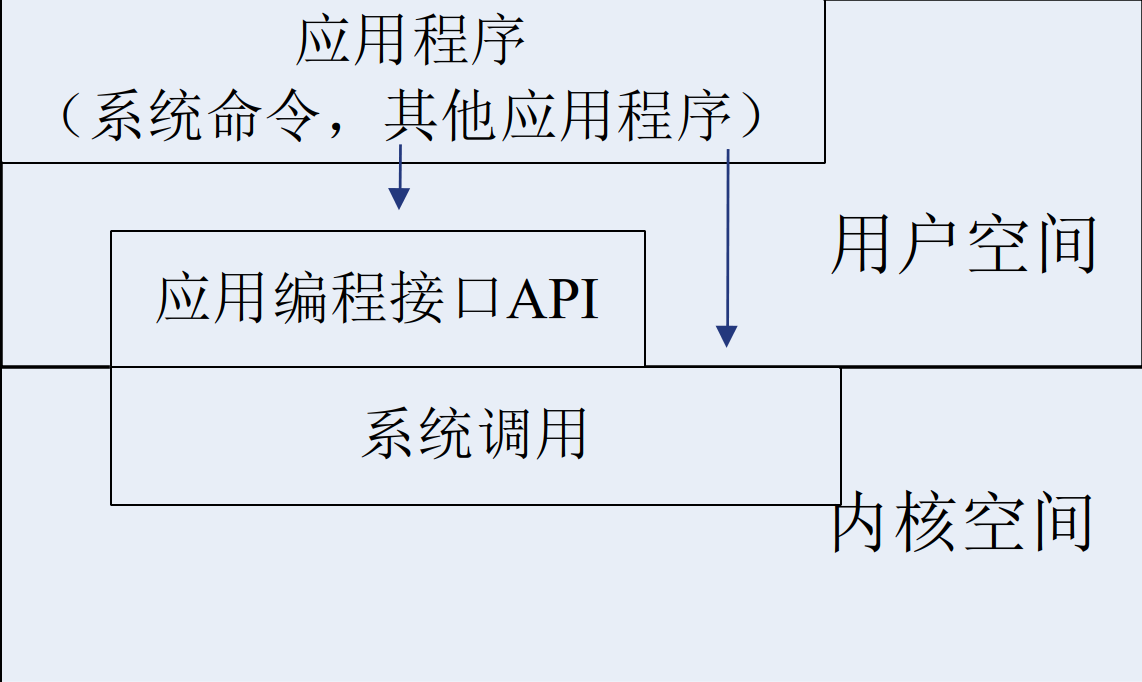
\includegraphics{./fig/linux1.png}}
 \caption{系统调用流程}
 \label{}
\end{figure}
\subsection{进程间通信}
    
进程间通信(IPC,Inter-Process Communication)指的是在同一操作系统中运行的不同进程之间传递信息或信号的机制。在Linux系统编程中,常见的IPC机制包括管道、信号、消息队列、共享内存、信号量等。
    
\subsection{线程}
    
线程是程序中的单一顺序控制流程,是操作系统能够进行运算调度的最小单位。它被包含在进程之中,是进程中的实际运作单位。同一进程内的多个线程将共享该进程的资源。多线程能提高程序的并发性,以提高应用程序的响应速度。在Linux中,线程是轻量级的进程,因此也拥有一些类似于进程的属性,但由于线程共享了进程的资源,所以线程之间的切换比进程之间的切换更加高效。

\subsection{Linux应用编程接口API}

Linux应用编程接口(API,Application Programming Interface)是一系列函数和过程,允许创建的应用程序可以访问操作系统的特定功能和资源。Linux API提供了大量的库函数,用于实现各种任务,如文件操作、网络通信、内存管理等。这些库函数在程序调用时,最终都会被映射到具体的系统调用。
    
\subsubsection{请求机制}
    
请求API函数的过程通常包括创建一个包含特定参数的数据结构,然后调用与任务相对应的API函数。API函数会将参数数据结构传递给操作系统内核,内核再执行相应的系统调用。

\subsubsection{标准}
    
Linux API主要遵循两个标准:POSIX和GNU。POSIX(Portable Operating System Interface)是IEEE为了实现软件在UNIX操作系统间的可移植性而制定的一系列API标准。GNU库(Glibc)是GNU项目发布的用于提供系统调用的C库,它基本上遵循POSIX标准,但同时也提供了一些额外的API。
    
\subsubsection{实现方法}
    
Linux API的实现涉及到用户空间和内核空间的交互。当程序调用一个API函数时,该函数会创建一个系统调用,并将控制权交给操作系统。操作系统会切换到内核模式,执行系统调用,然后返回结果,最后再切换回用户模式。
    
\subsection{Linux系统命令}
    
Linux系统命令是在命令行接口(CLI)中执行操作的文本输入。Linux系统提供了大量的系统命令,用于执行各种任务,如文件操作(如ls、cd、mv等)、系统监控(如top、ps等)、网络工具(如ping、netstat等)等。在Linux系统编程中,可以通过系统调用来执行这些系统命令。每个系统命令都有一系列的选项和参数,可以用来定制命令的行为。

\section{文件及文件描述符}

\subsection{文件}

在Linux系统中,几乎所有的事物都可以被视为文件。这些包括硬件设备、目录,甚至是网络通信,它们在Linux中都可以被当作文件来处理。文件是一个包含数据的容器,数据可以以任何格式存储在文件中。文件包含两部分信息:用户数据和元数据。用户数据是文件的主体部分,元数据则包含了关于文件的信息,如文件的大小、创建和修改时间、所有者和权限等。

\textbf{Linux文件类型:普通文件、目录文件、链接文件、设备文件}

\subsection{文件描述符}

文件描述符是一个用于访问文件或者其他输入/输出资源,如管道或网络套接字的非负整数。在Linux系统中,文件描述符是在进程中创建的,并在进程的生命周期内使用。它们是由内核自动分配的,并且总是返回最小的未使用的文件描述符。例如,当进程打开一个现有文件或者创建一个新文件时,操作系统将返回一个文件描述符以供进程在后续操作中使用。

在每个进程启动时,它都会有三个已经打开的文件描述符。标准输入(STDIN)的文件描述符是0,标准输出(STDOUT)的文件描述符是1,以及标准错误(STDERR)的文件描述符是2。这些文件描述符通常连接到用户的终端。

在Linux系统编程中,有多种系统调用用于操作文件描述符,如open, read, write, close等。

\section{底层文件I/O操作}

\subsection{打开文件}

在Linux中,可以使用系统调用 open() 打开一个文件。该函数需要文件名和打开模式作为参数,如只读、只写或读写等。如果操作成功,open() 将返回一个文件描述符,它是一个小的非负整数,可以在程序中用于引用该打开的文件。如果出错,open() 将返回-1。

\begin{verbatim}
    #include <fcntl.h>
    int open(const char *path, int flags);
    int open(const char *path, int flags, mode_t mode);
\end{verbatim}

\subsection{读取文件}

读取文件是通过 read() 系统调用完成的。该函数需要文件描述符、数据缓冲区的地址和要读取的字节数作为参数。read() 返回实际读取的字节数,如果已经到达文件末尾,那么返回0,如果出现错误则返回-1。

\begin{verbatim}
    #include <unistd.h>
    ssize_t read(int fd, void *buf, size_t count);
\end{verbatim}

\subsection{写入文件}

向文件中写入数据是通过 write() 系统调用完成的。该函数需要文件描述符、数据缓冲区的地址和要写入的字节数作为参数。write() 返回实际写入的字节数,如果出现错误则返回-1。

\begin{verbatim}
    #include <unistd.h>
    ssize_t write(int fd, const void *buf, size_t count);
\end{verbatim}

\subsection{关闭文件}

关闭文件是通过 close() 系统调用完成的。该函数需要文件描述符作为参数,如果关闭操作成功,那么返回0,如果出现错误则返回-1。

\begin{verbatim}
    #include <unistd.h>
    int close(int fd);
\end{verbatim}

\subsection{定位文件读写位置}

通过 lseek() 系统调用可以在文件中改变当前的读写位置。该函数需要文件描述符、偏移量和基准点作为参数。如果操作成功,返回新的读写位置,如果出现错误则返回-1。

\begin{verbatim}
    #include <unistd.h>
    off_t lseek(int fd, off_t offset, int whence);
\end{verbatim}


\subsection{文件锁}

在Linux中,可以使用文件锁(File Lock)来实现对文件的互斥访问。文件锁分为共享锁(Shared Lock)和独占锁(Exclusive Lock),用于控制对文件的读写操作。

\subsubsection{设置文件锁}

文件锁的设置使用 fcntl() 系统调用。通过设置 F_SETLK 或 F_SETLKW 命令,可以获取或释放文件锁。

\begin{verbatim}
#include <fcntl.h>
int fcntl(int fd, int cmd, struct flock *lock);
\end{verbatim}

其中,fd 是文件描述符,cmd 是命令,lock 是指向 struct flock 结构的指针,该结构定义了文件锁的类型和位置。在设置文件锁时,需要设置以下字段:

\begin{itemize}
\item l_type:锁的类型,可以是 F_RDLCK(共享锁)或 F_WRLCK(独占锁)。
\item l_whence:偏移量的基准点,可以是 SEEK_SET、SEEK_CUR 或 SEEK_END。
\item l_start:锁定区域的起始偏移量。
\item l_len:锁定区域的长度。
\end{itemize}

\subsubsection{测试文件锁}

文件锁的测试使用 fcntl() 系统调用。通过设置 F_GETLK 命令,可以检测给定的锁是否会阻塞。

\begin{verbatim}
#include <fcntl.h>
int fcntl(int fd, int cmd, struct flock *lock);
\end{verbatim}

其中,fd 是文件描述符,cmd 是命令,lock 是指向 struct flock 结构的指针。在测试文件锁时,需要设置以下字段:

\begin{itemize}
\item l_type:锁的类型,可以是 F_RDLCK(共享锁)或 F_WRLCK(独占锁)。
\item l_whence:偏移量的基准点,可以是 SEEK_SET、SEEK_CUR 或 SEEK_END。
\item l_start:锁定区域的起始偏移量。
\item l_len:锁定区域的长度。
\end{itemize}

\subsubsection{释放文件锁}

文件锁的释放使用 fcntl() 系统调用。通过设置 F_SETLK 命令,并将锁的类型设置为 F_UNLCK,可以释放文件锁。

\begin{verbatim}
#include <fcntl.h>
int fcntl(int fd, int cmd, struct flock *lock);
\end{verbatim}

其中,fd 是文件描述符,cmd 是命令,lock 是指向 struct flock 结构的指针。在释放文件锁时,需要设置以下字段:

\begin{itemize}
\item l_type:锁的类型,设置为 F_UNLCK。
\item l_whence:偏移量的基准点,可以是 SEEK_SET、SEEK_CUR 或 SEEK_END。
\item l_start:锁定区域的起始偏移量。
\item l_len:锁定区域的长度。
\end{itemize}

文件锁对于控制多个进程对同一文件的并发访问非常有用,可以防止数据损坏或不一致性。


\subsection{例程:copyfile.c}

该程序复制源文件(src_file)的最后1024字节(或少于1024字节,如果源文件小于1024字节)到目标文件(dest_file)。

\begin{minted}{c}
#include <unistd.h>  // 提供对POSIX操作系统API的访问,如文件处理和进程管理。
#include <fcntl.h>   // 提供文件控制操作,如打开和修改文件。
#include <stdio.h>   // 提供基本的输入输出功能。
#include <stdlib.h>  // 提供了一些通用函数,如内存管理,程序的退出等。

#define OFFSET 1024      // 定义偏移量,用于指定需要复制的文件部分的大小。
#define SRC_FILE "src"   // 定义源文件名。
#define DEST_FILE "dest" // 定义目标文件名。
#define BUFFER_SIZE 1024 // 定义缓冲区的大小。

int main(){
    int src_fd, dest_fd;  // 定义源文件和目标文件的文件描述符。
    unsigned char buff[BUFFER_SIZE];  // 定义缓冲区,用于存储文件读取的数据。
    int real_read_len;  // 定义实际读取的字节数。
    // 以只读方式打开源文件。
    src_fd = open(SRC_FILE, O_RDONLY);
    // 以写入方式打开目标文件,如果文件不存在则创建,如果文件已存在则清空文件内容。
    dest_fd = open(DEST_FILE, O_WRONLY|O_CREAT
                   |O_TRUNC, S_IRUSR|S_IWUSR|S_IRGRP|S_IROTH);
    // 检查文件是否正确打开。
    if (src_fd<0||dest_fd<0){
        // 如果打开文件失败,输出错误信息并退出程序。
        perror("Open file error");
        exit(1);
    }
    // 输出源文件和目标文件的文件描述符。
    printf("src fd:%d, dest fd:%d\n",src_fd,dest_fd);

    // 将源文件的读写位置定位到文件的末尾减去OFFSET处。
    if (lseek(src_fd, -OFFSET, SEEK_END)<0){
        // 如果定位失败,输出错误信息并退出程序。
        perror("Lseek error");
        exit(-1);
    }
    // 从源文件中读取数据,并写入到目标文件中。
    while((real_read_len=read(src_fd,buff,sizeof(buff)))>0){
        // 如果写入的字节数不等于读取的字节数,输出错误信息并退出程序。
        if (write(dest_fd, buff, real_read_len)!=real_read_len){
            perror("Write file error");
            exit(-1);
        }
    }        
    // 关闭源文件和目标文件。
    close(src_fd);
    close(dest_fd);
    return 0;  // 程序正常结束。
}

\end{minted}
\section{标准I/O编程}

\subsection{概述}

Linux标准I/O库提供了一组函数,用于读写流,这些函数比系统调用更易于使用。在C语言中,标准I/O库被包含在stdio.h头文件中。

\subsection{标准I/O函数}

\subsubsection{读函数}

\begin{itemize}
    \item \texttt{fgetc}: 从流中获取下一个字符。
    \item \texttt{fgets}: 从流中获取下一行。
    \item \texttt{fread}: 从流中读取数据。
\end{itemize}

\subsubsection{写函数}

\begin{itemize}
    \item \texttt{fputc}: 向流中写入一个字符。
    \item \texttt{fputs}: 向流中写入一个字符串。
    \item \texttt{fwrite}: 向流中写入数据。
\end{itemize}

\subsection{缓冲}

标准I/O库使用缓冲来减少读写操作的数量。这意味着当你调用一个写函数时,数据可能不会立即写入磁盘,而是存储在缓冲区中,等待缓冲区满了或者你显式地刷新缓冲区。

标准I/O提供3种类型的缓冲存储:

\subsubsection{全缓冲}

在这种阻塞I/O模型中,填满标准I/O缓存后才进行实际I/O操作。

\subsubsection{行缓冲}

这是一种非阻塞模型,在输入和输出中遇到行结束符时,标准I/O库执行I/O操作。

\subsubsection{不带缓冲}

相当于用系统调用write()函数将这些字符全写到被打开的文件上。例如,stderr是不带缓冲的。

\subsection{文件定位}

可以使用\texttt{fseek}、\texttt{ftell}和\texttt{rewind}函数来在流中更改和查询位置。

\subsection{错误处理}

如果一个标准I/O函数遇到错误,它会设置全局变量\texttt{errno},你可以使用\texttt{perror}或\texttt{strerror}函数来获取错误信息。

\section{Linux进程概述}

\subsection{进程的概念与结构}
在Linux中,进程是一个运行的程序实例,具有自己的地址空间和状态。它的行为由进程控制块(Process Control Block,PCB)控制,其中包含了进程标识、状态、用户标识、资源利用情况等信息。

\subsubsection{程序/进程}
程序是一组指示计算机执行特定任务的指令,而进程则是程序的一个活动实例。程序只是硬盘上的一组指令,而进程则包括程序的代码、当前状态和运行时的数据。

\subsubsection{进程控制块PCB}
进程控制块(PCB)是用于存储进程相关信息的数据结构。这些信息包括:进程标识、程序计数器、CPU寄存器、CPU调度信息、内存管理信息、进程的状态等。

\subsubsection{进程标识}
进程标识包括进程号(PID,Process Identity Number)和父进程号(PPID,parent process ID)。PID和PPID都是非零的正整数,它们可以唯一地标识一个进程。在Linux中,可以使用系统调用函数getpid()和getppid()来获取当前进程的PID和PPID。

\subsubsection{其他参数}
PCB中还包含其他一些参数,如:用户/用户组标识,进程时间,资源利用情况等。

\subsection{进程的状态}
一个进程在其生命周期中可能会有几种状态,包括就绪态、执行态、等待态、暂停态、僵尸态。

\subsubsection{就绪态}
在就绪态下,进程具备执行的一切条件,正在等待分配CPU的处理时间片。

\subsubsection{执行态}
在执行态下,进程正在运行,即进程正在占用CPU。

\subsubsection{等待态}
在等待态下,进程不能使用CPU,若等待事件发生(等待的资源分配到)则可将其唤醒。

\subsubsection{暂停态}
在暂停态下,进程暂停执行,通常是因为收到了一个信号。

\subsubsection{僵尸态}
僵尸进程是已经终止,但其父进程还没有获取其终止状态的进程。在Linux中,僵尸进程无法被杀死,因为它已经"死亡",只是其退出状态还未被父进程读取。

\begin{figure}[H]
\centering
 \resizebox{0.75\textwidth}{!}{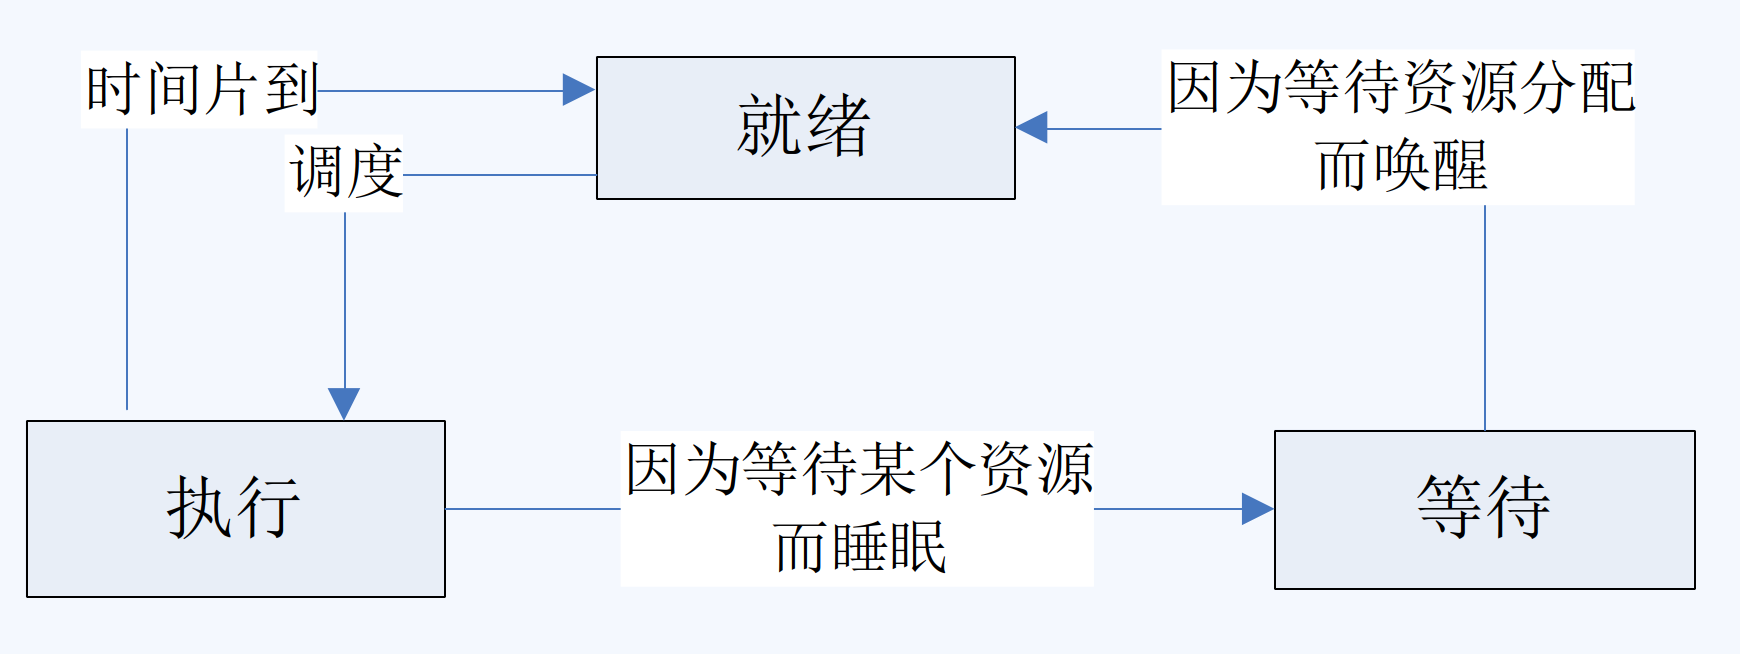
\includegraphics{./fig/process1.png}}
 \caption{Linux进程状态转换图}
 \label{}
\end{figure}

\subsection{进程地址空间}
进程之间具有并行性,互不干扰,每个进程运行在独立的虚拟地址空间。这个地址空间主要分为三个段:数据段,代码段和堆栈段。

\subsubsection{数据段}
数据段用于存放进程运行中需要的数据。它进一步分为两个部分:普通数据段和BSS数据段。普通数据段存放静态初始化的全局变量或常量,而BSS数据段存放未初始化的全局变量。

\subsubsection{代码段}
代码段包含进程执行的机器指令。

\subsubsection{堆栈段}
堆栈段是进程中动态分配的内存区域,通常用于存放局部变量和程序调用的返回地址。

\begin{figure}[H]
\centering
 \resizebox{0.5\textwidth}{!}{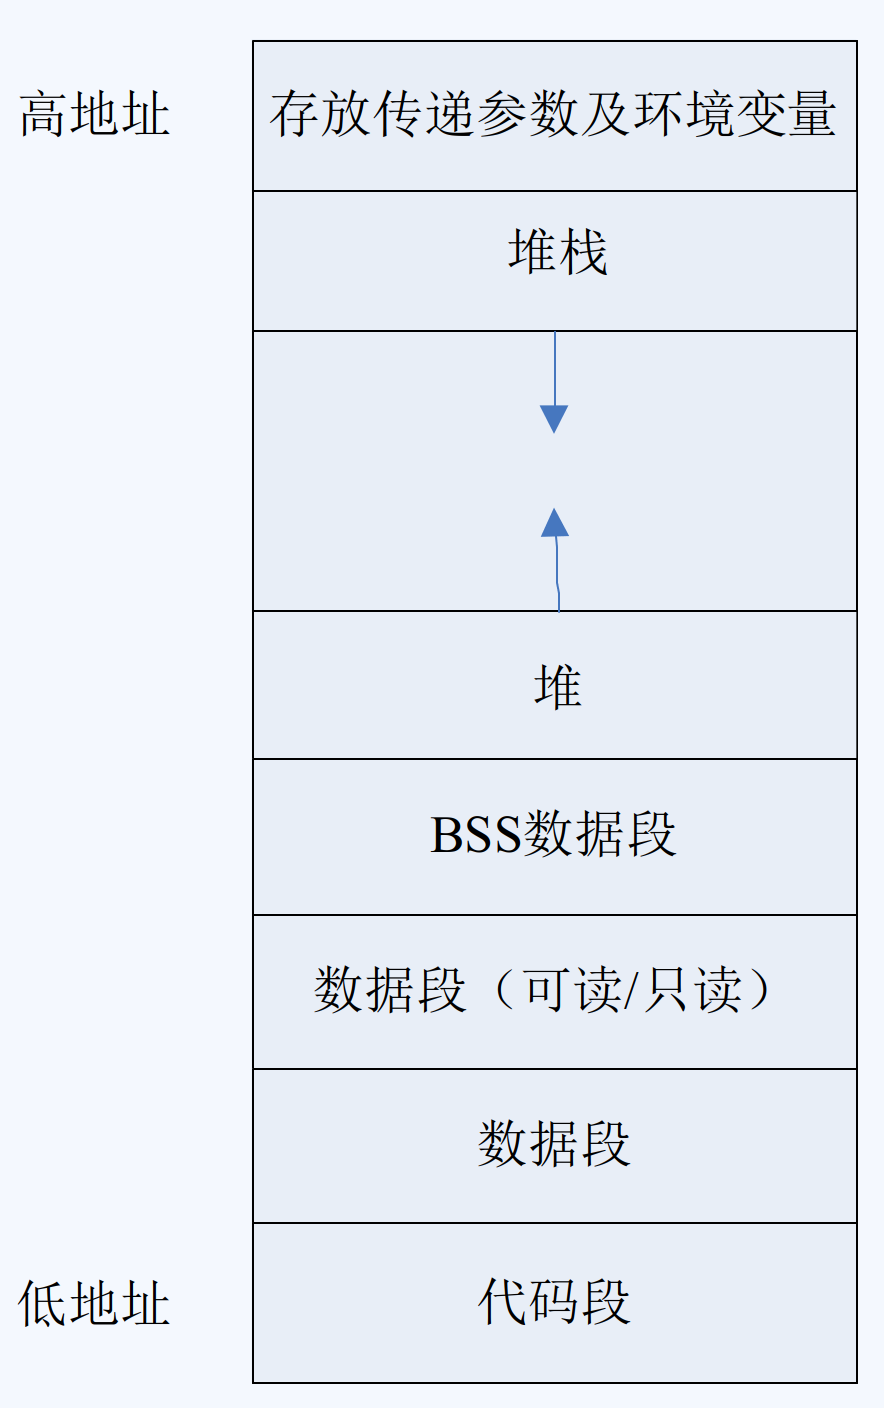
\includegraphics{./fig/process2.png}}
 \caption{进程地址空间}
 \label{}
\end{figure}

\subsection{进程管理}
进程的管理涵盖了进程的启动、调度和中断等方面的操作。

\subsubsection{启动进程}
进程可以通过以下方式启动:
\begin{itemize}
    \item 手工启动:用户可以手动启动一个进程,这可以分为前台启动和后台启动。前台启动的进程会占用控制台,而后台启动的进程则不会。后台启动一般用于进程耗时长,或者用户不急于获得结果的情况。
    \item 调度启动:系统也可以根据用户的设置或事先的调度安排自行启动进程。
\end{itemize}

\subsubsection{调度进程}
进程调度是操作系统的核心功能之一。它负责决定哪个进程能够获得CPU的使用权,以及进程何时可以从一个状态转换到另一个状态。通过进程调度,我们可以实现对进程的中断操作,改变进程的优先级,以及查看进程的状态等。

\subsection{进程控制}
进程的创建、管理和终止都在进程控制部分完成。下面我们将详细地介绍这些操作。

\subsubsection{创建新进程:fork()函数}
在Linux中,创建新的进程通常使用fork()函数。它从当前进程(被称为父进程)创建一个新的进程(被称为子进程)。子进程是父进程的复制品,它继承了父进程的地址空间,包括数据空间、堆和栈的副本。但是,子进程有自己的进程号、资源使用和计时器等。

子进程和父进程的执行是并行的,从fork()函数的返回开始,它们分别在各自的地址空间中运行。通过检查fork()函数的返回值,可以判断是在父进程中还是在子进程中。在父进程中,返回值是子进程的进程号,而在子进程中,返回值是0。

\subsubsection{查询子进程是否终止:wait和waitpid函数}
当进程正常或异常终止时,内核会向其父进程发送SIGCHLD信号。父进程可以调用wait或waitpid函数来查询其子进程是否已经终止。

wait函数使父进程阻塞,直到一个子进程结束。如果子进程已经结束,wait函数将立即返回。

waitpid函数与wait函数的作用相同,但是它提供了一些额外的功能。首先,它提供了一个非阻塞的版本的wait函数。其次,它并不一定要等待第一个结束的子进程,它可以等待一个特定的子进程。

\begin{verbatim}
pid_t fork(void);
pid_t wait(int *status);
pid_t waitpid(pid_t pid, int *status, int options);
\end{verbatim}


\subsection{例程: wait_list.c}

该例程主要演示了如何创建子进程,然后通过父进程等待子进程的退出。

\begin{minted}{c}
#include <stdio.h>   // 提供基本的输入输出功能。
#include <stdlib.h>  // 提供了一些通用函数,如内存管理,程序的退出等。
#include <sys/types.h> // 为了使用pid_t类型。
#include <unistd.h>  // 提供对POSIX操作系统API的访问,如文件处理和进程管理。
#include <sys/wait.h> // 提供进程等待的函数。

int main(){
    pid_t pid,pw;  // 定义进程ID。
    int status;  // 定义子进程的状态。

    // 创建新的进程。fork函数返回两次:一次在父进程中,返回子进程的PID;一次在子进程中,返回0。
    if ((pid=fork())<0){
        // 如果创建进程失败,输出错误信息并退出程序。
        perror("fork");
        exit(-1);
    }else if (pid==0){
        // 子进程的代码。
        printf("In child process: %d\n",getpid());  // 输出子进程的PID。
        sleep(5);  // 使子进程暂停5秒。
        exit(1);  // 子进程退出,返回状态1。
    }else{
        // 父进程的代码。
        printf("In parent process:\n");  // 输出父进程的提示信息。
        do{
            // 使用非阻塞方式等待子进程的结束。如果子进程没有结束,返回0。
            pw=waitpid(pid,&status,WNOHANG);
            if (pw==0){
                // 如果子进程还没有结束,输出提示信息并暂停1秒。
                printf("No child exit.\n");
                sleep(1);
            }
        }while(pw==0);  // 如果子进程还没有结束,继续等待。

        // 当子进程结束时,输出子进程的PID和退出状态。
        printf("Child %d exit, exit status:%d.\n",pw,WEXITSTATUS(status));
    }

    return 0;  // 程序正常结束。
}
\end{minted}

\subsection{特殊进程}
\subsubsection{孤儿进程}
孤儿进程是父进程先退出,而它的一个或多个子进程还在运行时产生的。这些子进程将成为孤儿进程。为了保证子进程能找到一个新的父亲,孤儿进程将被init进程(进程号为1)所收养,并由init进程对它们完成状态收集工作。孤儿进程不会额外占用系统资源。

\begin{figure}[h]
    \centering
    \begin{tikzpicture}
        % Nodes
        \node[draw] (parent) at (0,0) {父进程};
        \node[draw] (child) at (4,0) {子进程};
        \node[draw] (orphan) at (4,-2) {孤儿进程};
        \node[draw] (init) at (8,-2) {init进程};
        
        % Arrows
        \draw[->] (parent) -- node[above] {导致} (child);
        \draw[->] (child) -- node[left]{转为}(orphan);
        \draw[->] (orphan) -- node[above]{回收}(init);
    \end{tikzpicture}
    \caption{孤儿进程}
    \end{figure}

\subsubsection{僵尸进程}
僵尸进程是子进程比父进程先结束,而父进程没有回收子进程时产生的。僵尸进程仅仅在进程列表中保留一个位置,记载该进程的退出状态等信息供其他进程收集,除此之外不再占有任何内存空间。然而,系统所能使用的进程号是有限的,如果大量的产生僵尸进程,将因为没有可用的进程号而导致系统不能产生新的进程。父进程可以通过wait或waitpid函数来等待子进程结束,以此清除僵尸进程。

流程图:父进程 --> 子进程结束 --> 产生僵尸进程 --> 父进程使用wait/waitpid函数 --> 清除僵尸进程

\section{进程间通信编程}

\subsection{Linux进程间通信概述}
在Linux系统中,进程可以使用多种方法进行通信,以实现数据的传递和同步。下面是一些常用的Linux进程间通信机制:

\subsubsection{管道}
管道是一种简单而常见的进程间通信方式。在Linux中,管道可以分为无名管道和有名管道(FIFO)两种类型。无名管道只能用于具有亲缘关系的父子进程之间的通信,而有名管道允许不相关的进程之间进行通信。

\subsubsection{信号量}
信号量是一种用于进程间同步和互斥的机制。它基于一个计数器和一组操作,进程可以对信号量进行等待、增加或减少操作。信号量可以用于控制对共享资源的访问,以避免竞争条件和死锁。

\subsubsection{共享内存}
共享内存是一种高效的进程间通信机制,它允许多个进程共享同一块内存区域。这种共享内存区域可以被进程直接读取和写入,从而实现进程之间的快速数据交换。但是,由于没有内置的同步机制,进程必须使用其他方式来确保数据的一致性和互斥。

\subsection{管道}
管道是Linux中的一种进程间通信方式,主要用于具有亲缘关系的进程之间的通信。管道具有以下特点:
\begin{itemize}
    \item 管道是一种半双工通信模式。
    \item 管道可以看作是一种特殊的文件,在内核的内存空间中创建和关闭。
    \item 管道基于文件描述符,创建管道时会生成两个文件描述符fd[0]和fd[1]。
    \item fd[0]用于读取管道,fd[1]用于写入管道。
\end{itemize}

\subsubsection{创建管道}
使用pipe()函数可以创建一个管道,步骤如下:
\begin{enumerate}
    \item 调用pipe()函数创建管道。
    \item 使用fork()函数创建子进程,该子进程会继承父进程所创建的管道。
\end{enumerate}

\subsubsection{父子进程之间的管道通信}
在父子进程之间建立了管道后,可以通过关闭不相关的文件描述符来实现读写操作。这样,父子进程之间就建立起了一条“子进程写入父进程读取”的通道。

\subsubsection{有名管道}
有名管道(FIFO)用于使互不相关的两个进程彼此通信。以下是有名管道的一些特点:
\begin{itemize}
    \item 有名管道通过路径名在文件系统中可见。
    \item 使用mkfifo()函数可以创建有名管道。
    \item 有名管道遵循先进先出规则,读取操作总是从开始处返回数据,写入操作将数据添加到末尾。
    \item 有名管道不支持像lseek()等文件定位操作。
    \item 可以使用open()、read()和write()等函数对有名管道进行读写操作。
\end{itemize}

\subsubsection{阻塞与非阻塞操作}
在管道的读写操作中,可能会出现阻塞的情况。可以使用阻塞和非阻塞的打开模式来控制管道的行为:
\begin{itemize}
    \item 对于读进程:
    \begin{itemize}
        \item 如果管道是阻塞打开且内部没有数据,则读进程将一直阻塞,直到有数据可读。
        \item 如果管道是非阻塞打开,不论管道内是否有数据,读进程都会立即执行读操作,如果管道内没有数据,读函数将立即返回0。
    \end{itemize}
    \item 对于写进程:
    \begin{itemize}
        \item 如果管道是阻塞打开,写操作将一直阻塞,直到数据可以被写入。
        \item 如果管道是非阻塞打开,写操作可能进行部分写入或调用失败,具体取决于管道的状态。
    \end{itemize}
\end{itemize}

\subsection{信号量}
在多个进程同时运行且彼此存在关联时,同步关系和互斥关系变得重要。这些关系的根源在于临界资源,即在同一时刻只允许有限个(通常只有一个)进程访问或修改的资源。临界资源可以是硬件资源(如处理器、内存、存储器和外围设备等),也可以是软件资源(如共享代码段、共享结构和变量等)。临界区本身也可以成为临界资源。

信号量是一种用于解决进程之间同步和互斥的进程间通信(IPC)机制。它基于一个称为信号量的变量,该变量对应于某种资源,并取一个非负整数值。信号量的值表示当前可用的该资源数量,若值为0,则表示当前没有可用的资源。同时,等待该资源的进程会进入信号量的等待队列。

信号量操作有两个原子操作,即P操作和V操作。P操作(也称为减操作)会使信号量的值减少,若减为负值,则当前进程会被阻塞。V操作(也称为增操作)会使信号量的值增加,若增加后的值大于0,则会唤醒等待队列中的某个进程。

以下是使用信号量访问临界区的伪代码:
\begin{verbatim}
P(semaphore)          // 进入临界区之前的操作
临界区操作
V(semaphore)          // 离开临界区之后的操作
\end{verbatim}

最简单的信号量是二值信号量,即只能取0和1两种值。信号量的创建和操作可以通过以下函数实现:

\subsubsection{semget()函数定义:}
\begin{verbatim}
#include <sys/types.h>
#include <sys/ipc.h>
#include <sys/sem.h>
int semget(key_t key, int nsems, int semflg);
\end{verbatim}
\emph{返回值:成功时返回信号量标识符(非负整数),失败时返回-1。}

\subsubsection{semctl()函数定义:}
\begin{verbatim}
#include <sys/types.h>
#include <sys/ipc.h>
#include <sys/sem.h>
int semctl(int semid, int semnum, int cmd, ...);
\end{verbatim}
\emph{返回值:成功时返回操作的结果,失败时返回-1。}

\subsubsection{semop()函数定义:}
\begin{verbatim}
#include <sys/types.h>
#include <sys/ipc.h>
#include <sys/sem.h>
struct sembuf {
    unsigned short sem_num;
    short sem_op;
    short sem_flg;
};
int semop(int semid, struct sembuf *sops, size_t nsops);
\end{verbatim}
\emph{返回值:成功时返回0,失败时返回-1。}

\subsection{共享内存}
共享内存是一种高效的进程间通信方式,它允许进程直接读写内存而无需进行数据的拷贝。以下是共享内存的相关概念和步骤:

共享内存是为了在多个进程间交换信息而在内核中留出的一块内存区域。进程可以将这块内存映射到自己的私有地址空间中,从而直接读写该内存区域,提高了通信效率。

多个进程共享同一段内存时,需要使用某种同步机制,例如互斥锁和信号量,来确保数据的一致性和互斥访问。

\subsubsection{共享内存编程步骤}
使用共享内存进行进程间通信的步骤如下:

1. \textbf{创建共享内存}:使用shmget()函数从内核中获取一段共享内存区域。
   \begin{itemize}
       \item \textbf{函数原型}:int shmget(key_t key, size_t size, int shmflg);
       \item \textbf{参数}:key为共享内存的键值,size为共享内存的大小,shmflg为创建共享内存的权限和标志。
       \item \textbf{返回值}:返回共享内存的标识符(shmid)。
   \end{itemize}
   
2. \textbf{映射共享内存}:使用shmat()函数将创建的共享内存映射到具体的进程地址空间中。
   \begin{itemize}
       \item \textbf{函数原型}:void *shmat(int shmid, const void *shmaddr, int shmflg);
       \item \textbf{参数}:shmid为共享内存的标识符, shmaddr为映射到进程地址空间的地址, shmflg为映射共享内存的权限和标志。
       \item \textbf{返回值}:返回共享内存的起始地址。
   \end{itemize}

3. \textbf{使用共享内存}:可以使用不带缓冲的I/O读写命令对共享内存进行操作。

4. \textbf{撤销映射操作}:使用shmdt()函数将共享内存从当前进程的地址空间中撤销映射。
   \begin{itemize}
       \item \textbf{函数原型}:int shmdt(const void *shmaddr);
       \item \textbf{参数}:shmaddr为共享内存的起始地址。
       \item \textbf{返回值}:返回0表示成功,-1表示失败。
   \end{itemize}

5. \textbf{删除共享内存}:使用shmctl()函数删除共享内存。
   \begin{itemize}
       \item \textbf{函数原型}:int shmctl(int shmid, int cmd, struct shmid_ds *buf);
       \item \textbf{参数}:shmid为共享内存的标识符,cmd为删除共享内存的命令,buf为用于存储共享内存信息的结构体指针。
       \item \textbf{返回值}:返回0表示成功,-1表示失败。
   \end{itemize}

\subsection{例程:sem_com.c}
这段代码定义了一些用于操作信号量的函数和一个用于存储信号量控制命令的联合类型 semun。

这些函数用于操作信号量,其中:

·init_sem 函数用于初始化信号量,并将初始值设置为 init_value。

·del_sem 函数用于删除信号量。

·sem_p 函数执行 P 操作(等待),将信号量的值减一。

·sem_v 函数执行 V 操作(释放),将信号量的值加一。

这些函数通过系统调用 semctl 和 semop 来进行信号量的控制操作,并使用 perror 函数输出错误信息并退出程序(使用 -1 表示错误)。

\begin{minted}{c}
union semun {
    int val;                  // 信号量值
    struct semid_ds *buf;     // IPC_STAT 和 IPC_SET 使用的缓冲区
    unsigned short *array;    // GETALL 和 SETALL 使用的数组
};
// 初始化信号量
int init_sem(int sem_id, int init_value) {
    union semun sem_union;
    sem_union.val = init_value;  // 设置信号量初始值
    // 设置信号量的值h
}
// P操作(等待)
int sem_p(int sem_id) {
    struct sembuf sem_buf;
    sem_buf.sem_num = 0;    // 信号量的编号(只有一个信号量时为0)
    sem_buf.sem_op = -1;    // P操作的值为-1,表示等待
    sem_buf.sem_flg = SEM_UNDO;  // 设置SEM_UNDO标志,保证进程终止时会释放占用的资源
    // 执行P操作
    if (semop(sem_id, &sem_buf, 1) == -1) {
        perror("sem p");  // 输出错误信息
        exit(-1);         // 退出程序
    }
    return 0;
}
// V操作(释放)
int sem_v(int sem_id) {
    struct sembuf sem_buf;
    sem_buf.sem_num = 0;    // 信号量的编号(只有一个信号量时为0)
    sem_buf.sem_op = 1;     // V操作的值为1,表示释放
    sem_buf.sem_flg = SEM_UNDO;  // 设置SEM_UNDO标志,保证进程终止时会释放占用的资源
    // 执行V操作
    if (semop(sem_id, &sem_buf, 1) == -1) {
        perror("sem v");  // 输出错误信息
        exit(-1);         // 退出程序
    }
    return 0;
}
\end{minted}

\subsection{例程:sem_2.c}
这段代码展示了使用信号量实现进程间同步的例子。该程序创建了一个信号量,并使用信号量实现了父子进程之间的同步。父进程和子进程在关键位置执行P操作和V操作,保证了它们的顺序执行。父进程和子进程都在延迟后正常退出,并在最后删除了信号量。
\begin{minted}{c}
#include <stdio.h>   // 提供基本的输入输出功能。
#include <stdlib.h>  // 提供了一些通用函数,如内存管理,程序的退出等。
#include <unistd.h>  // 提供对POSIX操作系统API的访问,如文件处理和进程管理。
#include <sys/sem.h> // 提供信号量相关的函数和数据结构。
#include "sem_com.c"  // 引入信号量的初始化、删除、P操作和V操作函数的定义。
#include <sys/types.h>  // 提供了一些基本类型的定义。
#include <sys/ipc.h>  // 提供了一些与IPC相关的函数和数据结构。

#define DELAY_TIME 3  // 定义延迟时间,单位为秒。

int main(){
    pid_t pid;  // 定义进程ID。
    int sem_id;  // 定义信号量ID。
    key_t sem_key;  // 定义信号量的键值。

    sem_key = ftok(".", 'b');  // 使用当前目录和字符 'b' 生成信号量的键值。
    if ((sem_id = semget(sem_key, 1, 0666|IPC_CREAT)) == -1) {
        perror("sem get");  // 输出错误信息
        exit(-1);  // 退出程序
    }
    init_sem(sem_id, 1);  // 初始化信号量,初始值为1。
    if ((pid = fork()) < 0) {
        perror("fork");  // 输出错误信息
        exit(1);  // 退出程序
    } else if (pid == 0) {
        sem_p(sem_id);  // 执行P操作
        printf("1.In child process:\n");  // 输出子进程的提示信息。
        sleep(DELAY_TIME);  // 使子进程暂停指定的延迟时间。
        printf("2.Child pid:%d\n", getpid());  // 输出子进程的PID。
        sem_v(sem_id);  // 执行V操作
        exit(0);  // 子进程正常退出,返回状态0。
    } else {
        sem_p(sem_id);  // 执行P操作
        printf("3.In parent process:\n");  // 输出父进程的提示信息。
        sleep(DELAY_TIME);  // 使父进程暂停指定的延迟时间。
        printf("4.Parent pid:%d\n", getpid());  // 输出父进程的PID。
        sem_v(sem_id);  // 执行V操作
        waitpid(pid, 0, 0);  // 等待子进程结束
        del_sem(sem_id);  // 删除信号量
        exit(0);  // 父进程正常退出,返回状态0。
    }
    return 0;  // 程序正常结束。
}

\end{minted}

\subsection{例程:shm_test.c}
这段代码展示了使用共享内存进行进程间通信的例子,使用共享内存实现了父子进程之间的通信。父进程创建了一个共享内存,然后等待用户输入一条消息,并将该消息复制到共享内存中。子进程在一定延迟后附加到共享内存并读取其中的数据。父子进程都在最后分离共享内存,父进程删除共享内存。

\begin{minted}{c}
#include <stdio.h>   // 提供基本的输入输出功能。
#include <stdlib.h>  // 提供了一些通用函数,如内存管理,程序的退出等。
#include <string.h>  // 提供了一些字符串处理函数。
#include <sys/types.h>  // 提供了一些基本类型的定义。
#include <unistd.h>  // 提供对POSIX操作系统API的访问,如文件处理和进程管理。
#include <sys/ipc.h>  // 提供了一些与IPC相关的函数和数据结构。
#include <sys/shm.h>  // 提供了共享内存相关的函数和数据结构。

#define DELAY_TIME 10  // 定义延迟时间,单位为秒。
#define SIZE 2048  // 定义共享内存的大小。

int main(){
    pid_t pid;  // 定义进程ID。
    int shmid;  // 定义共享内存ID。
    char *shm_addr;  // 定义共享内存的起始地址。
    char buff[SIZE];  // 定义缓冲区用于存储数据。

    // 创建共享内存
    if ((shmid = shmget(IPC_PRIVATE, SIZE, 0666)) < 0) {
        perror("shmget");  // 输出错误信息
        exit(-1);  // 退出程序
    } else {
        printf("Create shared memory: %d.\n", shmid);  // 输出共享内存的ID
    }

    // 创建子进程
    if ((pid = fork()) < 0) {
        perror("fork");  // 输出错误信息
        exit(1);  // 退出程序
    } else if (pid == 0) {
        sleep(DELAY_TIME);  // 子进程暂停一段时间

        printf("1.In child process:\n");
        // 将共享内存附加到子进程的地址空间
        if ((shm_addr = shmat(shmid, 0, 0)) == (void*)-1) {
            perror("shmat");  // 输出错误信息
            exit(-1);  // 退出程序
        }

        strcpy(buff, shm_addr);  // 将共享内存中的数据复制到缓冲区
        printf("Child receive: %s\n", buff);  // 输出子进程接收到的数据

        // 分离共享内存
        if (shmdt(shm_addr) < 0) {
            perror("shmdt");  // 输出错误信息
            exit(-1);  // 退出程序
        }
        exit(0);  // 子进程正常退出,返回状态0。
    } else {
        printf("In parent process:\n");
        // 将共享内存附加到父进程的地址空间
        if ((shm_addr = shmat(shmid, 0, 0)) == (void*)-1) {
            perror("shmat");  // 输出错误信息
            exit(-1);  // 退出程序
        }

        printf("\nInput msg:\n");
        fgets(buff, SIZE, stdin);  // 从标准输入读取数据到缓冲区
        strncpy(shm_addr, buff, strlen(buff));  // 将缓冲区的数据复制到共享内存

        // 分离共享内存
        if (shmdt(shm_addr) < 0) {
            perror("shmdt");  // 输出错误信息
            exit(-1);  // 退出程序
        }

        waitpid(pid, NULL, 0);  // 等待子进程结束

        // 删除共享内存
        if (shmctl(shmid, IPC_RMID, NULL) == -1) {
            perror("shmctl");  // 输出错误信息
            exit(-1);  // 退出程序
        }

        exit(0);  // 父进程正常退出,返回状态0。
    }

    return 0;  // 程序正常结束。
}

\end{minted}

\section{Linux多线程编程}

\subsection{线程概述}

\subsubsection{进程与线程}
进程是系统中程序执行和资源分配的基本单位。每个进程都有自己的数据段、代码段和堆栈段。在进行切换时,需要有比较复杂的上下文切换。

线程减少处理机的空转时间,支持多处理器以及减少上下文切换开销, 比创建进程小很多。线程是进程内独立的一条运行路线,是处理器调度的最小单元,也称为轻量级进程。线程可以对进程的内存空间和资源进行访问,并与同一进程中的其他线程共享线程。线程相关的执行状态和存储变量放在线程控制表内。一个进程可以有多个线程,有多个线程控制表及堆栈寄存器,共享一个用户地址空间。

\subsubsection{线程标识}
线程ID是一个重要的概念,每个线程都有一个唯一的线程ID。进程ID在整个系统中是唯一的,而线程ID只在它所属的进程环境中有效。

\begin{itemize}
    \item 函数: pthread\_self() 

    原型: \texttt{pthread\_t pthread\_self(void);} 

    参数: 无

    返回值: 调用线程的线程ID

    \item 函数: pthread\_equal() 

    原型: \texttt{int pthread\_equal(pthread\_t t1, pthread\_t t2);} 

    参数: t1, t2 -- 需要比较的两个线程ID

    返回值: 如果两个线程ID相等,则返回非零值,否则返回0
\end{itemize}

\subsection{线程编程}

\subsubsection{创建线程}
线程创建后,就开始运行相关的线程函数。创建线程我们一般使用pthread_create()函数。

\subsubsection{退出线程}
在线程函数运行完后,该线程也就退出了。或者我们也可以使用pthread_exit()函数主动使线程退出。需要注意的是,我们不能使用exit()函数,因为它会使调用进程终止,导致所有线程都终止。

\subsubsection{等待线程}
由于一个进程中的多个线程是共享数据段的,通常在线程退出之后,退出线程所占用的资源并不会随着线程的终止而得到释放。我们通常使用pthread_join()函数来等待线程的结束。这个函数会将调用线程挂起,直到被等待的线程结束为止。函数返回时,被等待线程的资源就被收回。

\subsubsection{取消线程}
在一些情况下,我们可能需要在一个线程中终止另一个线程,我们可以使用pthread_cancel()函数来完成这个操作。被取消的线程可以设置自己的取消状态,决定是接受还是忽略这个取消请求。

\begin{itemize}
    \item 函数: pthread\_create() 

    原型: \texttt{int pthread\_create(pthread\_t *thread, const pthread\_attr\_t *attr, void *(*start\_routine) (void *), void *arg);}

    参数: thread -- 新线程的标识符指针;attr -- 线程属性设置,通常置为NULL表示使用默认属性;start\_routine -- 线程函数起始地址;arg -- 传给线程函数的参数

    返回值: 成功时返回0,错误时返回错误号

    \item 函数: pthread\_exit()

    原型: \texttt{void pthread\_exit(void *retval);}

    参数: retval -- 线程的返回值

    返回值: 无

    \item 函数: pthread\_join()

    原型: \texttt{int pthread\_join(pthread\_t thread, void **retval);}

    参数: thread -- 被等待的线程标识符;retval -- 用户定义的指针,用来存储被等待线程的返回值

    返回值: 成功时返回0,错误时返回错误号

    \item 函数: pthread\_cancel()

    原型: \texttt{int pthread\_cancel(pthread\_t thread);}

    参数: thread -- 被取消的线程标识符

    返回值: 成功时返回0,错误时返回错误号
\end{itemize}
\subsection{线程同步与互斥}

线程共享进程的资源和地址空间,对这些资源进行操作时,必须考虑线程间同步与互斥问题。通常我们有三种线程同步机制:互斥锁,信号量和条件变量。互斥锁更适合同时可用的资源是惟一的情况,而信号量更适合同时可用的资源为多个的情况。

\subsubsection{互斥锁}
互斥锁用简单的加锁方法控制对共享资源的原子操作。只有两种状态: 上锁、解锁。我们可以把互斥锁看作某种意义上的全局变量。在同一时刻只能有一个线程掌握某个互斥锁,拥有上锁状态的线程能够对共享资源进行操作。如果其他线程希望上锁一个已经被上锁的互斥锁,那么该线程就会挂起,直到上锁的线程释放掉互斥锁为止。互斥锁保证让每个线程对共享资源按顺序进行原子操作。

\subsubsection{信号量}
信号量是操作系统中所用到的PV原子操作,广泛用于进程或线程间的同步与互斥。信号量本质上是一个非负的整数计数器,被用来控制对公共资源的访问。一次P操作使信号量减一,而一次V操作使信号量加一。进程(或线程)根据信号量的值来判断是否对公共资源具有访问权限。当信号量的值大于等于零时,该进程(或线程)具有公共资源的访问权限。当信号量的值小于零时,该进程(或线程)就将阻塞直到信号量的值大于等于0为止。PV操作主要用于线程间的同步和互斥。如果需要实现互斥,几个线程只设置一个信号量;如果需要实现同步,会设置多个信号量,安排不同初值来实现它们之间的顺序执行。

信号量相关的函数有:
\begin{itemize}
    \item 函数: sem\_init(sem\_t *sem, int pshared, unsigned int value) 

    创建一个信号量,并初始化它。第一个参数是指向信号量对象的指针,第二个参数指示信号量是在进程内部还是进程间共享,第三个参数是信号量的初始值。

    \item 函数: sem\_wait(sem\_t *sem) 和 sem\_trywait(sem\_t *sem)

    这两个函数都是用于P操作,在信号量大于零时将信号量的值减一。若信号量小于零时,sem\_wait()将会阻塞线程,sem\_trywait()则会立即返回。

    \item 函数: sem\_post(sem\_t *sem)

    用于V操作,将信号量的值加一同时发出信号来唤醒等待的线程。

    \item 函数: sem\_getvalue(sem\_t *sem, int *valp)

    用于获取信号量的值,将信号量的当前值放入valp指向的整数中。

    \item 函数: sem\_destroy(sem\_t *sem)

    用于删除信号量,使信号量失效并释放其占用的系统资源。
\end{itemize}


\subsection{线程技术发展}
在Linux 2.2内核中,不存在真正意义上的线程。Linux 2.4内核消除了线程个数的限制,允许动态地调整进程数上限。在Linux 内核2.6之前,进程是最主要的处理调度单元,并没支持内核线程机制。Linux 2.6内核实现了共享地址空间的进程机制,在1996年第一次获得线程的支持。

为了改善LinuxThread问题,根据新内核机制重新编写线程库,改善Linux对线程的支持。由IBM主导的新一代POSIX线程库(Next Generation POSIX Threads,简称为NGPT)项目在2002年启动。为了避免出现有多个Linux线程标准,在2003年停止该项目。由Red Hat主导的本地化POSIX线程库 (Native POSIX Thread Library,简称为NTPL) 最早在Red Hat Linux9中被支持。现在已经成为GNU C函数库的一部分,同时也成为Linux线程的标准.

\subsection{例程:thread_sem.c}
这是一个使用 POSIX 线程(pthreads)和信号量(semaphores)来同步线程执行的 C 语言程序

\begin{minted}{c}
#include <stdio.h>     //包含了基础的输入输出函数,比如printf
#include <stdlib.h>    //包含了一些标准库函数,比如exit和rand
#include <pthread.h>   //包含了pthread库,用于多线程编程
#include <semaphore.h> //包含了信号量操作的函数
                       //比如sem_init, sem_wait和sem_post

#define NUM 3          //定义了常量NUM,表示线程数
#define JOBS 5         //定义了常量JOBS,表示每个线程执行的任务数
#define DELAY 5        //定义了常量DELAY,表示任务延迟的最大值

sem_t sem[NUM];        //声明了一个信号量数组,用于线程间的同步

//这是每个线程要执行的函数
void *thrd_func(void *arg){
    long int seq = (long int)arg;   //获取线程序号
    int delay_time =0;
    int i;

    sem_wait(&sem[seq]);            //线程在开始执行前等待对应的信号量

    printf("Thread %d is running.\n",seq);   //打印线程开始执行的信息   
    
    //模拟线程执行JOBS次任务
    for(i=0;i<JOBS;i++){
        delay_time = (int)(DELAY*(rand()/(double)RAND_MAX))+1;   //随机生成延迟时间
        sleep(delay_time);                                       //模拟任务执行延迟
        printf("\tThread %d, job:%d, delay:%d.\n",seq, i,delay_time);   //打印任务执行信息
    }

    printf("Thread %d finished.\n",seq);   //打印线程完成的信息
    
    sem_post(&sem[(seq+NUM-1)%NUM]);       //线程执行完毕后,释放前一个线程的信号量
    return 0;
}

int main(){
    pthread_t tid[NUM];      //声明一个线程ID数组,用于存储每个线程的ID
    long int no;
    int i;

    srand((int)time(0));     //初始化随机数生成器

    sem_init(&sem[0],0,0);   //初始化信号量,设置初始值为0
    sem_init(&sem[1],0,0);   
    sem_init(&sem[2],0,1);   //初始化信号量,设置初始值为1

    //创建NUM个线程
    for(no=0;no<NUM;no++){    
        if (pthread_create(&tid[no], NULL, thrd_func, (void*)no) !=0 ){   
            perror("pthread create");   //打印创建线程失败的错误信息
            exit(-1);                   //创建线程失败时退出程序
        }
        printf("Create thead %d.\n",no);   //打印创建线程的信息
    }

    //等待所有线程执行完毕
    for(no=0;no<NUM;no++){    
        if (pthread_join(tid[no],NULL)!=0){
            perror("pthread exit");    //打印线程退出失败的错误信息
            exit(-1);                  //线程退出失败时退出程序
        }
    }
    
    //销毁信号量
    for(i=0;i<NUM;i++)
        sem_destroy(&sem[i]);   

    return 0;
}

\end{minted}

\section{综合实例}

\subsection{例程:shared\_memory.c}
该程序创建了一个子进程,父进程和子进程之间通过共享内存和信号量进行通信。父进程从终端读取用户输入的数据,然后将数据拷贝到共享内存中,然后释放信号量sem_1。子进程等待信号量sem_1,当sem_1的值大于0时,子进程将共享内存中的数据拷贝到本地缓冲区,并打印接收到的数据,然后释放信号量sem_2。父进程再次等待信号量sem_2,当sem_2的值大于0时,父进程删除共享内存段和信号量,并等待子进程退出,最后父进程退出。

\begin{minted}{c}
#include <stdio.h>          //包含了基础的输入输出函数,比如printf
#include <stdlib.h>         //包含了一些标准库函数,比如exit
#include <string.h>         //包含了一些字符串处理函数,比如strcpy和strlen
#include <sys/types.h>      //包含了一些系统调用的数据类型定义,比如pid_t
#include <unistd.h>         //包含了一些系统调用函数,比如fork和getpid
#include <sys/ipc.h>        //包含了一些共享内存和信号量的相关定义,比如IPC_PRIVATE
#include <sys/shm.h>        //包含了一些共享内存操作函数,比如shmget和shmat
#include "sem_com.c"        //包含了信号量操作的函数,比如create_sem和sem_p

#define SIZE 2048           //定义共享内存的大小

int main(){
    pid_t pid;
    int shmid;
    char *shm_addr;
    int sem_1,sem_2;
    char buff[SIZE];

    sem_1= create_sem('a');     //创建信号量sem_1
    sem_2= create_sem('b');     //创建信号量sem_2
    init_sem(sem_1,0);          //初始化信号量sem_1为0,表示初始状态下不可用
    init_sem(sem_2,1);          //初始化信号量sem_2为1,表示初始状态下可用

    shmid=shmget(IPC_PRIVATE, SIZE, 0666);    //创建共享内存段,返回共享内存的标识符
    printf("Create shared memory: %d.\n",shmid);


    if ((pid=fork())<0){        //创建子进程
        perror("fork");         //打印fork失败的错误信息
        exit(1);                //fork失败时退出程序
    }else if (pid==0){          //子进程执行以下代码
        printf("In child process:\n");

        sem_p(sem_1);           //等待信号量sem_1,如果sem_1的值大于0,则减1并继续执行,否则阻塞等待
        shm_addr=shmat(shmid,0,0);   //将共享内存连接到子进程的地址空间中

        strcpy(buff,shm_addr);       //将共享内存中的数据拷贝到本地缓冲区
        printf("Child receive:%s\n",buff);   //打印接收到的数据

        shmdt(shm_addr);             //将共享内存从子进程的地址空间中分离
        sem_v(sem_2);                //释放信号量sem_2,将其值加1

        exit(0);                     //子进程退出
    }else{                          //父进程执行以下代码
        printf("In parent process:\n");
        
        sem_p(sem_2);                //等待信号量sem_2,如果sem_2的值大于0,则减1并继续执行,否则阻塞等待
        shm_addr=shmat(shmid,0,0);    //将共享内存连接到父进程的地址空间中

        printf("\nInput msg:\n");    
        fgets(buff,SIZE,stdin);      //从终端读取用户输入的数据
        strncpy(shm_addr,buff,strlen(buff));   //将数据拷贝到共享内存中

        shmdt(shm_addr);             //将共享内存从父进程的地址空间中分离

        sem_v(sem_1);                //释放信号量sem_1,将其值加1

        waitpid(pid,NULL,0);         //等待子进程退出

        shmctl(shmid,IPC_RMID,NULL); //删除共享内存段

        del_sem(sem_1);              //删除信号量sem_1
        del_sem(sem_2);              //删除信号量sem_2

        exit(0);                     //父进程退出
    }

    return 0;
}

\end{minted}

\subsection{例程:producer\_consumer.c}
该程序模拟了生产者消费者问题。生产者线程生产数据项并将其放入一个缓冲区中,消费者线程从缓冲区中取出数据项进行消费。缓冲区是一个固定大小的数组,使用循环队列的方式实现。生产者和消费者之间通过信号量进行同步,保证生产者在缓冲区未满时才能生产数据,消费者在缓冲区非空时才能消费数据。

具体流程如下:

\begin{itemize}
    \item 主函数创建了一个生产者线程和一个消费者线程。
    \item 初始化互斥信号量\texttt{lock}为1,表示互斥访问缓冲区的锁。
    \item 初始化生产者信号量\texttt{sem\_p}为缓冲区的大小\texttt{SIZE},表示生产者可生产的空闲位置数。
    \item 初始化消费者信号量\texttt{sem\_c}为0,表示初始状态下缓冲区没有可消费的数据。
    \item 生产者线程不断循环生产数据项:
    \begin{itemize}
        \item 等待生产者信号量\texttt{sem\_p},确保有可用的空闲位置。
        \item 申请互斥锁\texttt{lock},保护对缓冲区的互斥访问。
        \item 打印当前生产的数据项。
        \item 将数据项放入缓冲区,并更新写索引。
        \item 释放互斥锁\texttt{lock}。
        \item 增加消费者信号量\texttt{sem\_c},表示有可消费的数据。
        \item 休眠2秒,模拟生产过程的耗时。
    \end{itemize}
    \item 消费者线程不断循环消费数据项:
    \begin{itemize}
        \item 等待消费者信号量\texttt{sem\_c},确保有可消费的数据。
        \item 申请互斥锁\texttt{lock},保护对缓冲区的互斥访问。
        \item 从缓冲区读取数据项,并清空读取位置。
        \item 更新读索引。
        \item 打印当前消费的数据项。
        \item 释放互斥锁\texttt{lock}。
        \item 增加生产者信号量\texttt{sem\_p},表示有可生产的空闲位置。
        \item 休眠1秒,模拟消费过程的耗时。
    \end{itemize}
    \item 主函数使用\texttt{pthread\_join}等待生产者和消费者线程退出。
    \item 销毁信号量,释放资源。
\end{itemize}

\begin{minted}{c}
#include <stdio.h>     //包含了基础的输入输出函数,比如printf
#include <stdlib.h>    //包含了一些标准库函数,比如exit和rand
#include <string.h>    //包含了一些字符串处理函数,比如memset
#include <pthread.h>   //包含了pthread库,用于多线程编程
#include <semaphore.h> //包含了信号量操作的函数,
                       //比如sem_init, sem_wait和sem_post

#define SIZE 5          //定义了缓冲区的大小

int buf[SIZE];          //声明了一个缓冲区数组
int write_index = 0;    //写索引
int read_index = 0;     //读索引
int idx = 0;            //数据项的值
sem_t lock;             //互斥信号量,用于保护对缓冲区的互斥访问
sem_t sem_c, sem_p;     //信号量,用于控制生产者和消费者之间的同步

//生产者线程函数
void *produce(void *arg){
    while(1){
        sem_wait(&sem_p);       //等待生产者信号量
        sem_wait(&lock);        //申请互斥访问缓冲区的锁
        
        printf("Produce: %d\n",idx);   //打印当前生产的数据项
        buf[write_index] = idx;        //将数据项放入缓冲区
        idx++;                         //递增数据项的值
        
        write_index = (write_index+1)%SIZE;   //更新写索引

        sem_post(&lock);               //释放缓冲区的互斥锁
        sem_post(&sem_c);              //增加消费者信号量       
        sleep(2);                      //休眠2秒,模拟生产过程的耗时
    }    
   
    return 0;
}

//消费者线程函数
void *consume(void *arg){
    int data;

    while(1){
        sem_wait(&sem_c);      //等待消费者信号量
        sem_wait(&lock);       //申请互斥访问缓冲区的锁
        
        data = buf[read_index];      //从缓冲区读取数据项
        buf[read_index] = -1;        //将读取的位置清空
        read_index = (read_index+1)%SIZE;   //更新读索引
        printf("Consume: %d\n",data);   //打印当前消费的数据项

        sem_post(&lock);               //释放缓冲区的互斥锁
        sem_post(&sem_p);              //增加生产者信号量       
        sleep(1);                      //休眠1秒,模拟消费过程的耗时
    }    
   
    return 0;
}

int main(){
    pthread_t con,pros;       //声明消费者线程和生产者线程的ID

    sem_init(&lock,0,1);      //初始化互斥信号量,设置初始值为1
    sem_init(&sem_p,0,SIZE);  //初始化生产者信号量,设置初始值为SIZE
    sem_init(&sem_c,0,0);     //初始化消费者信号量,设置初始值为0
    
    pthread_create(&pros, NULL, produce, NULL);   //创建生产者线程
    pthread_create(&con, NULL, consume, NULL);    //创建消费者线程

    pthread_join(con,0);     //等待消费者线程退出
    pthread_join(pros,0);    //等待生产者线程退出

    sem_destroy(&lock);      //销毁互斥信号量
    sem_destroy(&sem_p);     //销毁生产者信号量
    sem_destroy(&sem_c);     //销毁消费者信号量

    return 0;
}

\end{minted}

\chapter{Android应用程序开发}
\section{Java 基础 (类的扩展,声明和实例化,内部方法重写)}
类的扩展(继承)是 Java 的一个基本概念。我们创建一个新的类时,可以从一个已存在的类继承属性和方法。例如:

\begin{minted}{java}
public class Animal {
    public void eat() {
        System.out.println("Eating...");
    }
}

public class Dog extends Animal {
    // 在这里,Dog 类继承了 Animal 类的所有属性和方法,例如 eat() 方法。
    // 同时,我们可以在 Dog 类中添加新的方法或者重写从 Animal 类继承的方法。
    
    @Override
    public void eat() {
        System.out.println("Dog is eating...");
    }
}

\end{minted}

\section{安卓项目结构}
一个标准的 Android 项目包括以下基本结构:
\begin{enumerate}
    \item \textbf{\textit{app/src/main/java}}:包含应用的源代码 (.java 或 .kt 文件)
    \item \textbf{\textit{app/src/main/res}}:包含所有的资源文件,例如图片(res/drawable),布局(res/layout),值(res/values)等等
    \item \textbf{\textit{app/src/main/AndroidManifest.xml}}:Android 应用的配置文件,包含了应用需要的权限声明,注册的 Activity,Service 等信息
    \item \textbf{\textit{app/build.gradle}}:包含应用的编译配置信息,例如 target SDK version,dependencies 等
\end{enumerate}

\section{线性布局,相对布局的使用}
在 Android 中,你可以使用不同类型的布局来安排界面元素。比如:
\begin{enumerate}
    \item \textbf{\textit{线性布局(LinearLayout)}}:将元素按照垂直或者水平方向排列。
    \item \textbf{\textit{相对布局(RelativeLayout)}}:可以指定元素相对于其他元素或者父元素的位置
\end{enumerate}

\textbf{\textit{LinearLayout}} 的示例:
\begin{minted}[frame=lines,linenos,mathescape]{xml}
<LinearLayout
    android:layout_width="match_parent"
    android:layout_height="match_parent"
    android:orientation="vertical">

    <TextView
        android:layout_width="match_parent"
        android:layout_height="wrap_content"
        android:text="Text 1"/>

    <TextView
        android:layout_width="match_parent"
        android:layout_height="wrap_content"
        android:text="Text 2"/>

</LinearLayout>




\end{minted}

\textbf{\textit{RelativeLayout}} 的示例:
\begin{minted}[frame=lines,linenos,mathescape]{xml}
<RelativeLayout
    android:layout_width="match_parent"
    android:layout_height="match_parent">

    <TextView
        android:id="@+id/textView1"
        android:layout_width="wrap_content"
        android:layout_height="wrap_content"
        android:text="Text 1"/>

    <TextView
        android:layout_width="wrap_content"
        android:layout_height="wrap_content"
        android:text="Text 2"
        android:layout_below="@id/textView1"/>

</RelativeLayout>

\end{minted}
\section{TextView、Button 和 EditText的静态和动态使用}
\subsection{静态使用}
\begin{minted}[frame=lines,linenos,mathescape]{xml}
<TextView
    android:id="@+id/textView"
    android:layout_width="wrap_content"
    android:layout_height="wrap_content"
    android:text="Hello World!" />

<Button
    android:id="@+id/button"
    android:layout_width="wrap_content"
    android:layout_height="wrap_content"
    android:text="Click me" />

<EditText
    android:id="@+id/editText"
    android:layout_width="match_parent"
    android:layout_height="wrap_content"
    android:hint="Enter something" />



\end{minted}

\subsection{动态使用}
\begin{minted}[frame=lines,linenos,mathescape]{java}
LinearLayout layout = findViewById(R.id.layout);

TextView textView = new TextView(this);
textView.setText("Hello World!");
layout.addView(textView);

Button button = new Button(this);
button.setText("Click me");
layout.addView(button);

EditText editText = new EditText(this);
editText.setHint("Enter something");
layout.addView(editText);



\end{minted}

\section{Activity}
Activity 的生命周期主要包含以下几个阶段:onCreate(), onStart(), onResume(), onPause(), onStop(), onDestroy()。

以下是一个使用 Intent 携带数据跳转 Activity 的示例:

\begin{minted}[frame=lines,linenos,mathescape]{java}
Intent intent = new Intent(this, SecondActivity.class);
intent.putExtra("key", "value");
startActivity(intent);

\end{minted}

在 SecondActivity 中,你可以通过以下方式获取数据:

\begin{minted}[frame=lines,linenos,mathescape]{java}
String value = getIntent().getStringExtra("key");
\end{minted}

\section{Service、IntentService}
\subsection{Service}
Service 是一个在后台运行的组件,可以执行长时间运行的操作。Service 分为两种类型:Started 和 Bound。

以下是启动一个普通的 Service 的示例:
\begin{minted}[frame=lines,linenos,mathescape]{java}
Intent intent = new Intent(this, MyService.class);
startService(intent);

\end{minted}

\subsection{IntentService}
IntentService 是 Service 的一个子类,它使用工作线程来处理所有启动请求。如果你不需要 Service 与其他组件交互,或者想要在服务完成后自动停止,那么可以使用 IntentService。

以下是启动一个 IntentService 的示例:

\begin{minted}[frame=lines,linenos,mathescape]{java}
Intent intent = new Intent(this, MyIntentService.class);
startService(intent);

\end{minted}

\section{广播接收器 BroadcastReceiver}

以下是创建一个 BroadcastReceiver 的示例:
\begin{minted}[frame=lines,linenos,mathescape]{java}
public class MyBroadcastReceiver extends BroadcastReceiver {
    @Override
    public void onReceive(Context context, Intent intent) {
        // 这里处理接收到的广播
    }
}

\end{minted}
然后在 AndroidManifest.xml 文件中注册:
\begin{minted}[frame=lines,linenos,mathescape]{xml}
<receiver android:name=".MyBroadcastReceiver">
    <intent-filter>
        <action android:name="com.example.MY_ACTION" />
    </intent-filter>
</receiver>

\end{minted}

发送广播的示例:
\begin{minted}[frame=lines,linenos,mathescape]{java}
Intent intent = new Intent();
intent.setAction("com.example.MY_ACTION");
sendBroadcast(intent);

\end{minted}

\section{SQLite 数据库的增、删、改、查}
在 Android 中,SQLite 是一种轻量级的数据库,我们通常使用 SQLiteOpenHelper 类来管理数据库的创建和版本管理。

以下是一个简单的示例:
\begin{minted}[frame=lines,linenos,mathescape]{java}
public class MyDatabaseHelper extends SQLiteOpenHelper {
    private static final String DB_NAME = "SampleDB";
    private static final int DB_VERSION = 1;
    
    public MyDatabaseHelper(Context context) {
        super(context, DB_NAME, null, DB_VERSION);
    }

    @Override
    public void onCreate(SQLiteDatabase db) {
        String CREATE_TABLE = "CREATE TABLE MyTable 
                               (id INTEGER PRIMARY KEY, name TEXT)";
        db.execSQL(CREATE_TABLE);
    }

    @Override
    public void onUpgrade(SQLiteDatabase db, int oldVersion, 
                          int newVersion) {
        // 如果数据库需要升级,你可以在这里处理
    }
}

\end{minted}

然后,你可以像下面这样使用这个数据库:

\begin{minted}[frame=lines,linenos,mathescape]{java}
MyDatabaseHelper dbHelper = new MyDatabaseHelper(this);
SQLiteDatabase db = dbHelper.getWritableDatabase();

// 插入数据
ContentValues values = new ContentValues();
values.put("id", 1);
values.put("name", "Tom");
db.insert("MyTable", null, values);

// 查询数据
Cursor cursor = db.query("MyTable", null, null, 
                                    null, null, null, null);

// 更新数据
ContentValues values = new ContentValues();
values.put("name", "Jerry");
db.update("MyTable", values, "id = ?", new String[] {"1"});

// 删除数据
db.delete("MyTable", "id = ?", new String[] {"1"});

\end{minted}

\section{基于文件流的文件读写}

以下是写入和读取文件的示例:

\begin{minted}[frame=lines,linenos,mathescape]{java}
// 写入文件
FileOutputStream fos = openFileOutput("myFile.txt", Context.MODE_PRIVATE);
fos.write("Hello World!".getBytes());
fos.close();

// 读取文件
FileInputStream fis = openFileInput("myFile.txt");
BufferedReader reader = new BufferedReader(
                        new InputStreamReader(fis));
String line = reader.readLine();
reader.close();

\end{minted}

\section{访问内置传感器}
以下是如何访问加速度计的示例:
\begin{minted}[frame=lines,linenos,mathescape]{java}
SensorManager sensorManager = (SensorManager) getSystemService(
                                Context.SENSOR_SERVICE);
Sensor accelerometer = sensorManager.getDefaultSensor(
                            Sensor.TYPE_ACCELEROMETER);

SensorEventListener listener = new SensorEventListener() {
    @Override
    public void onSensorChanged(SensorEvent event) {
        float x = event.values[0];
        float y = event.values[1];
        float z = event.values[2];
        // 这里处理加速度数据
    }

    @Override
    public void onAccuracyChanged(Sensor sensor, int accuracy) {
        // 这里处理传感器精度改变
    }
};

sensorManager.registerListener(listener, accelerometer, 
                               SensorManager.SENSOR_DELAY_NORMAL);

\end{minted}

\end{document}